\documentclass{supervision}
\usepackage{course}
\usepackage{enumitem}

\Supervision{5}

\begin{document}
  \begin{questions}
    %%%%%%%%%%%%%%%%%%%%%%%%%%%%%%%
    \section*{Topic 05 - Transport}
    %%%%%%%%%%%%%%%%%%%%%%%%%%%%%%%

    \question \textit{Transport flavours}
      \begin{parts}
        \part The User Datagram Protocol (UDP) is sometimes used instead of
          TCP. It provides very few features above those provided by IP.

          \begin{subparts}
            \subpart Give one feature provided by UDP but not by IP, and one
              provided by UDP but not by TCP.
              \begin{solution}
                Provides multiplexing/demultiplexing capabilities.

                % TODO: one provided by UDP
              \end{solution}
              % multiplexing/demultiplexing (UDP has port numbers) framing (UDP
              % delineates packets)
              %
              % a terrible checksum

            \subpart Explain the role of a port number in UDP. Why isn’t it
              the Process ID? Explain the relation between TCP and UDP port
              numbers.
              % demultiplexing/remultiplexing: more than one flow per IP
              % address processID would be less flexible obfuscating client
              % (OS) information with mechanics of identifying the end of a
              % service.
              \begin{solution}
                By using port numbers multiple flows can happen simulataneously
                from a single IP address. A single process might want multiple
                flows and thus using the process ID is not as flexible as
                assigning a port number.
                % TODO: last part
              \end{solution}


            \subpart Give three characteristics which might make an
              application protocol better suited to implementation over UDP
              than over TCP.
              \begin{solution}
                A real time stream (e.g. an online multiplayer game). If the
                packet is not delivered on time then retransmision is useless
                as the data is now stale.
              \end{solution}
              % short-lived interactions (request-response)
              % small message sizes
              % loss detected easily
              % avoiding rate adaptation (e.g. real-time transport)

          \end{subparts}
      \end{parts}

    \question \textit{Error control, ARQ}
      \begin{parts}
        \part Why do error control protocols for packet switched networks use
          error detecting codes but not error correcting codes?
          \begin{solution}
            In a packet switched network the link is likely to either be fairly
            reliable or lose packets. In the first case error correcting codes
            add more overhead than simply retransmitting the corrupted packet.
            In the second case, since the entire packet is lost the codes are
            useless.
          \end{solution}

        \part A transport protocol for packet-switched networks uses a
          “sliding window” Automatic Repeat reQuest (ARQ) scheme for error
          control and flow control.

          \begin{subparts}
            \subpart As well as error detecting codes, ARQ protocols use
              acknowledgments and timeouts to achieve error control. Briefly
              explain what these are, and how they are combined to achieve
              reliable transmission.
              \begin{solution}
                \begin{description}
                  \item[Acknowledgments] Acknowledgments are packets sent by
                    the reciever to confirm receipt of uncorrupted packets.
                  \item[Timeouts] In the context of an ARQ protocol, a timeout
                    is used to trigger retransmission (i.e. when it can be
                    assumed from the lack of an acknowledgment that the packet
                    was lost).
                \end{description}
                In TCP acknowledgements are sent with the byte offset for the
                next packet it is expecting. If the sender recieves 3 ACKS with
                the same byte offset then it assumes that this is due to a lost
                packet (rather than duplicated ACKS or just out of order
                packets) and this triggers fast retransmission.
              \end{solution}

            \subpart What \emph{two} error cases might cause a receiver to send
              a negative acknowledgment (NACK)? How are they detected? What
              happens if the NACK is lost?
              \begin{solution}
                NACKs can be sent for:
                \begin{itemize}
                  \item Out of sequence packets
                  \item If a received packet fails checksum verification
                \end{itemize}

                If a NACK is lost then the sender will retransmit when the
                timeout fires.
              \end{solution}

            \subpart In what circumstances will a receiver receive a packet
              with the same sequence number twice? What should it do in these
              circumstances?
              \begin{solution}
                This could be caused by:
                \begin{itemize}
                  \item A lost or delayed ACK which resulted in unnecessary
                    retransmission
                  \item A duplicated packet
                \end{itemize}
                In these circumstances it should simply discard the second.
              \end{solution}

            \subpart Given that the protocol provides bidirectional
              communication, what optimisation can be made in the
              implementation of acknowledgments to reduce the total number of
              packets sent?
              \begin{solution}
                The acknowledgment packets can be piggy-backed onto other
                packets.
              \end{solution}

            \subpart If two hosts are connected by a 100Mbps link with a
              round-trip time of 20ms, how big (in bytes) should the sliding
              window be to maximise link usage?
              \begin{solution}
                The bandwidth-delay product should be used:
                $\SI{100}{Mbps} \times \SI{20}{ms} = 2Mb \: (\SI{250}{bytes})$
              \end{solution}

            \subpart Give two reasons why, at a given time, the window size
              might be set to a smaller value.
              \begin{solution}
                \begin{itemize}
                  \item The receiver has limited the rate due to buffer
                    limitations.
                  \item There is contention for capacity (causing some packets
                    to be lost).
                \end{itemize}
              \end{solution}

          \end{subparts}

        \part Consider a sliding window protocol with a window size of $5$
          using cumulative ACKs.

          \begin{description}
            \item[Retransmissions] Retransmissions occur under two
              conditions:
              \begin{itemize}
                \item Reception of three duplicate ACKs (that is, three
                  identical ACKs after the initial ACK)
                \item Timeout after \SI{100}{ms} (timer starts at the beginning
                  of the packet transmission)
              \end{itemize}
            \item[Timing]
              \begin{itemize}
                \item Data packets have a transmission time of \SI{1}{ms}.
                \item ACK packets have zero transmission time.
                \item The link has a latency of \SI{10}{ms}.
                \item The source $A$ starts off by sending its first packet at
                  time $t=0$.
              \end{itemize}
          \end{description}

          \begin{subparts}
            \subpart Assume all packets are successfully delivered except the
              following:
              \begin{itemize}
                \item The first transmission of data packet $\#3$
                \item The ACK sent in response to the receipt of data packet
                  $\#6$
              \end{itemize}
              When is data packet $\#3$ first retransmitted (expressed in terms
              of msec after $t=0$)?
              \begin{solution}
                The last bit of data packet $\#1$ reaches the destination at
                $\SI{11}{ms}$ (\SI{1}{ms} for transmission and \SI{10}{ms} for
                latency).

                Similarly, the time for the other packets are \SI{12}{ms},
                \emph{N/A}, \SI{14}{ms} and \SI{15}{ms} respectively.

                The acknowledgment packets for data packets $\#1$, $\#2$, $\#4$
                and $\#5$ have sequence numbers $2$, $3$, $3$ and $3$ and
                arrive at times \SI{21}{ms}, \SI{22}{ms}, \SI{24}{ms} and
                \SI{25}{ms} respectively.

                When the acknowledgments for data packets $\#2$ and $\#3$
                reach the sender they trigger packets $6$ and $7$ to be sent.

                Packet $7$ reaches the reciever at time \SI{33}{ms} and thus
                the acknowledgment reaches the sender at \SI{43}{ms}. Since
                this is the third duplicate it triggers the retransmission.
              \end{solution}

            \subpart Consider the same scenario, but with everything
              successfully delivered except the following:
              \begin{itemize}
                \item The first transmission of data packet $\#3$
                \item The first transmission of data packet $\#5$
                \item The ACK sent in response to the receipt of data packet
                  $\#6$
              \end{itemize}

              When is data packet \#3 first retransmitted (expressed in terms
              of msec after $t=0$)?
              \begin{solution}
                  \begin{center}
                    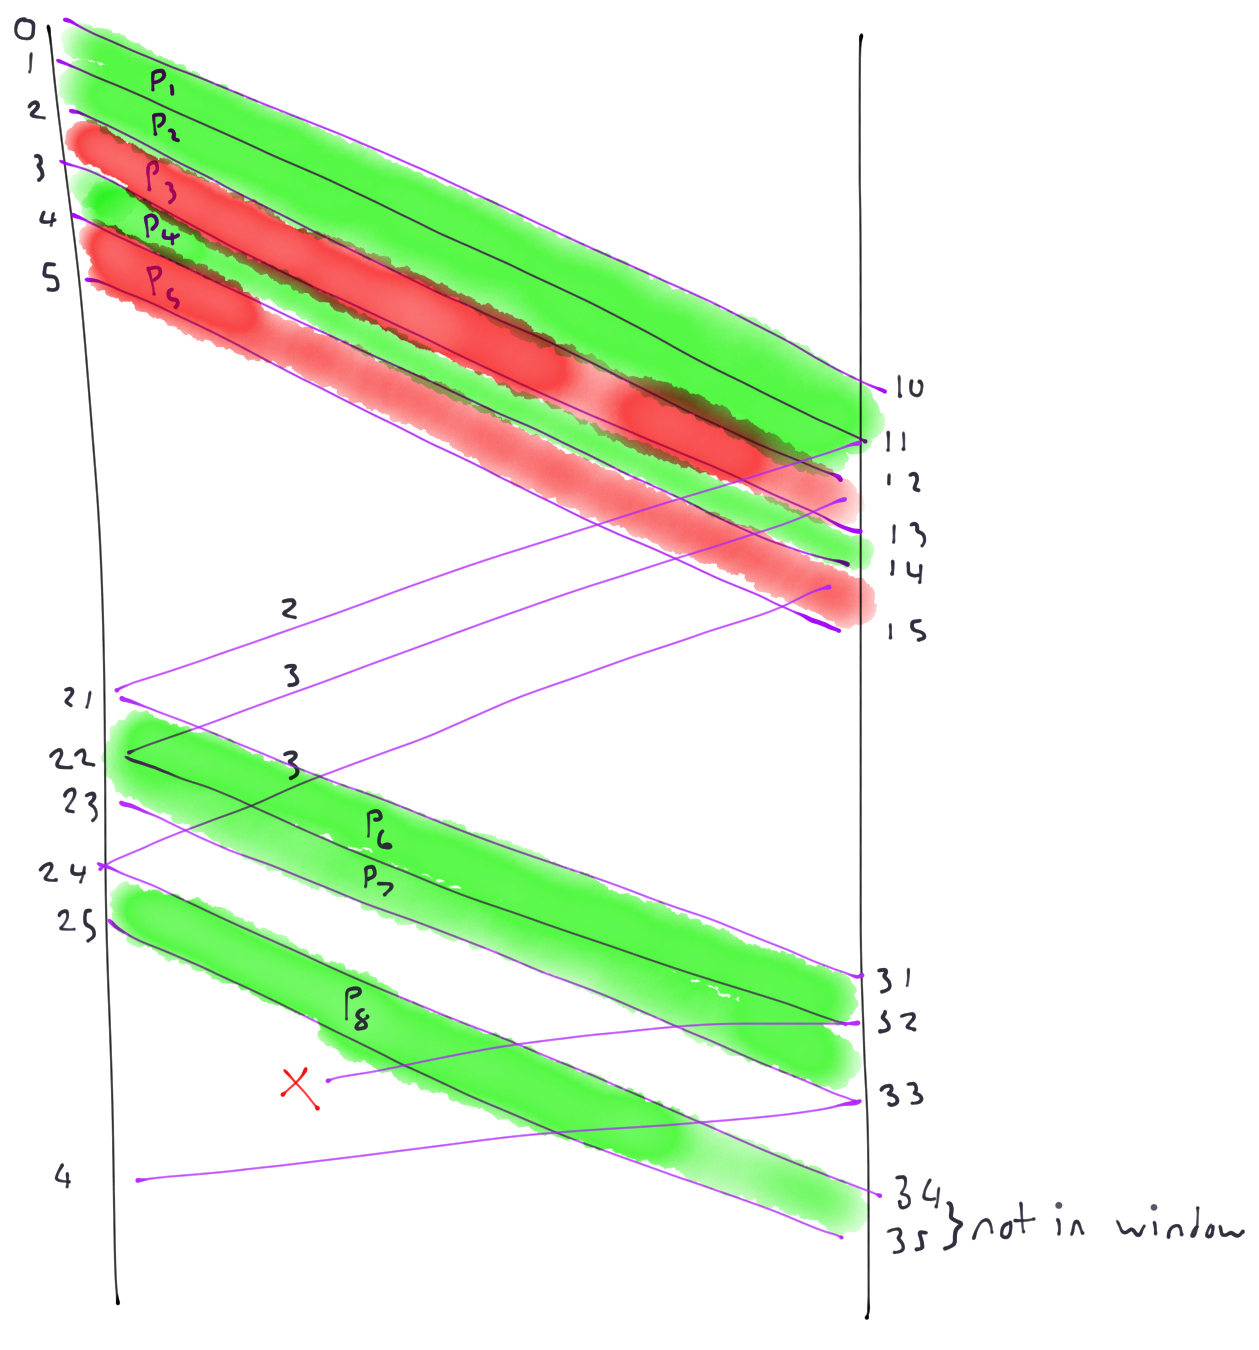
\includegraphics[width=0.8\textwidth]{5-transmission1}
                  \end{center}
                  No further transmission takes place until the timeout for
                  packet fires at \SI{102}{ms}
              \end{solution}

            \subpart Assume we can only observe the ACK packets arriving at
              the sender.

              The same sliding window algorithm is used, with the same
              timings and retransmission policies apply.

              Notation (read carefully): The notation $A_x$ is used to mean
              that the ACK packet is acknowledging the receipt of all packets
              up to and including data packet $x$.

              That is, $A_5$ is acknowledging the receipt of packet $5$; to be
              clear, the notation does not mean that the receiver is
              expecting packet $5$ as the next data packet.

              Assume that the following ACK packets arrive (just the ordering
              is shown, no timing information is provided):

              \begin{itemize}
                \item $A_1$
                \item $A_2$
                \item $A_3$
                \item $A_3$
                \item $A_4$
                \item $A_5$
                \item $A_6$
              \end{itemize}

              Which of the following five scenarios (described only by the
              unusual events that occurred; assume all else functioned
              normally) would have produced such a series of ACKs? (consider
              all that apply)

              \begin{enumerate}[label=(\alph*)]
                \item Data packet number $4$ was dropped
                \item Data packet number $4$ was delayed, arrived immediately
                  after data packet $5$
                \item Data packet $3$ was duplicated by the network
                \item ACK packet $A_3$ was duplicated by the network
                \item ACK packet $A_4$ was delayed, arriving after $A_5$
              \end{enumerate}
              \begin{solution}
                C and D apply.
              \end{solution}

            \subpart With the same set up as in the previous problem,
              consider the following stream of ACK packets.

              \begin{itemize}
                \item $A_1$
                \item $A_2$
                \item $A_3$
                \item $A_5$
                \item $A_4$
                \item $A_6$
              \end{itemize}

              Which of the following five scenarios (described only by the
              unusual events that occurred; assume all else functioned
              normally) would have produced such a series of ACKs? (consider
              all that apply)

              \begin{enumerate}[label=(\alph*)]
                \item Data packet number $4$ was dropped
                \item Data packet number $4$ was delayed, arrived immediately
                after data packet $5$
                \item Data packet $3$ was duplicated by the network
                \item ACK packet $A_3$ was duplicated by the network
                \item ACK packet $A_4$ was delayed, arriving after $A_5$
              \end{enumerate}
              \begin{solution}
                E is the only scanario that applies.
              \end{solution}

            \subpart With the same set up as in the previous problem,
              consider the following stream of ACK packets.

              \begin{itemize}
                \item $A_1$
                \item $A_2$
                \item $A_3$
                \item $A_3$
                \item $A_5$
                \item $A_6$
              \end{itemize}

              Which of the following five scenarios (described only by the
              unusual events that occurred; assume all else functioned
              normally) would have produced such a series of ACKs? (consider
              all that apply)

              \begin{enumerate}[label=(\alph*)]
                \item Data packet number $4$ was dropped
                \item Data packet number $4$ was delayed, arrived immediately
                after data packet $5$
                \item Data packet $3$ was duplicated by the network
                \item ACK packet $A_3$ was duplicated by the network
                \item ACK packet $A_4$ was delayed, arriving after $A_5$
              \end{enumerate}
              \begin{solution}
                B is the only scenario that applies.
              \end{solution}
          \end{subparts}
      \end{parts}

    \question \textit{TCP specifics}
      \begin{parts}
        \part Use the approximate equation for throughput as a function of
          drop rate:

          \begin{equation*}
            {throughput} = \frac{\sqrt{1.5} \times {MSS}}{RTT\sqrt{p}}
          \end{equation*}

          Assume an ${RTT}$ of \SI{40}{ms} and an ${MSS}$ of \SI{1000}{bytes}.
          In the following questions ignore IP and TCP headers in your
          calculations.

          \begin{subparts}
            \subpart What drop rate $p$ would lead to a throughput of
              \SI{1}{Gbps}?
              \begin{solution}
                Rearranging gives:
                \begin{equation*}
                  p = \left(
                    \frac{\sqrt{1.5} \times {MSS}}{RTT\times{throughput}}
                    \right)^2 = \num{6e-8}
                \end{equation*}
              \end{solution}

            \subpart What drop rate $p$ would lead to a throughput of
              \SI{10}{Gbps}?
              \begin{solution}
                Rearranging gives:
                \begin{equation*}
                  p = \left(
                    \frac{\sqrt{1.5} \times {MSS}}{RTT\times{throughput}}
                    \right)^2 = \num{6e-10}
                \end{equation*}
              \end{solution}

            \subpart If the connection is sending data at a rate of
              \SI{10}{Gbps}, how long on average is the time interval between
              drops?
              \begin{solution}
                The number of packets per second is given by:
                \begin{equation*}
                  \frac{{throughput}}{{MSS} \times 8}
                \end{equation*}
                Multiplying this by the drop rate gives you the number of
                packets dropped a second and the reciprical of this is the
                average time interval between dropped packets.
                \begin{equation*}
                  \frac{{MSS} \times 8}{{throughput} \times p} = \SI{1333}{s}
                \end{equation*}
              \end{solution}

            \subpart What window size $W$ (measured in terms of MSSes) would
              be required to maintain a sending rate of 10Gbps? (rounded down
              to the nearest integer)
              \begin{solution}
                The window size neccessary to fill the bandwidth-delay product
                is:
                \begin{equation*}
                  W = \frac{{throughput} \times {RTT}}{{MSS} \times 8} = 50,000
                \end{equation*}
              \end{solution}

            \subpart If a connection suffered a drop upon reaching 10Gbps,
              how long would it take for it to return to 10Gbps (after
              undergoing a fast retransmit)? (in seconds, rounded down to the
              nearest second)
              \begin{solution}

              \end{solution}

            \subpart Consider two TCP connections whose throughput obeys the
              TCP throughput equation listed above.

              The first TCP connection has the following parameters:
              ${MSS} = 1000 {bytes}$, ${RTT} = 0.2ms$, ${drop rate} = 0.5\%$

              The second TCP connection has the following parameters:
              ${MSS} = 2000 {bytes}$, ${RTT} = 0.1ms$, ${drop rate} = 8\%$

              What is the ratio of throughputs (the throughput of the first
              TCP connection divided by the throughput of the second TCP
              connection)? Why?
              \begin{solution}
                The ratio is $1$. Not sure how to justify this - I just plugged
                the numbers in.
              \end{solution}

          \end{subparts}

        \part Consider the plot of CWND versus time for a TCP connection.
          \begin{subparts}
            \subpart At each of marked marked points along the timeline in
              the figure on the next page, indicate what event has happened,
              or what phase of congestion control TCP is in (as appropriate),
              from the following set: Slow-Start, Congestion-Avoidance,
              Fast-Retransmit, and Timeout.
              \begin{solution}
                \begin{enumerate}[label=(\alph*)]
                  \item Slow-Start
                  \item Fast-Retransmit
                  \item Congestion-Avoidance
                  \item Fast-Retransmit
                  \item Congestion-Avoidance
                  \item Timeout
                  \item Slow-Start

                \end{enumerate}
              \end{solution}

            \subpart Assume CWND is $10,000$ right before $F$, what is the value
              of SSTHRESH at $G$?
              \begin{solution}
                $5,000$
              \end{solution}

          \end{subparts}
      \end{parts}
  \end{questions}
\end{document}
